\chapter{Dynamic Programming}



\section{Introduction}
The core philosophy of dp:
\begin{enumerate}
\item The definition of \textbf{states} 
\item The definition of the \textbf{transition functions} among states 
\end{enumerate} 

The so called concept dp as memoization of recursion does not grasp the core philosophy of dp. 

The formula in the following section are unimportant. Instead, what is important is the definition of dp array and transition function derivation.
\subsection{Common practice}
\runinhead{Dummy.} Use dummies to avoid using if-else conditional branch.
\begin{enumerate}
\item Use $n+1$ dp arrays to reserve space for dummies. 
\item Iteration range is $[1, n+1)$.
\item $n+k$ for k dummies  
\end{enumerate}
\runinhead{State definition.} Two general sets of state definitions - the state 
\begin{enumerate}
\item ends \textit{at} index $i$
\item ends \textit{before} index $i$
\item ends \textit{at} or \textit{before} index $i$
\end{enumerate}

\runinhead{Space optimization.} To avoid MLE, we need to carry out space optimization. Let $o$ be other subscripts, $f$ be the transition function. 

Firstly,
$$
F_{i, o} = f\big(F_{i-1, o'}\big)
$$

should be reduced to 
$$
F_{o} = f\big(F_{o'}\big)
$$

Secondly,
$$
F_{i, o} = f\big(F_{i-1, o'}, F_{i-2. o'}\big)
$$

should be reduced to 
$$
F_{i, o} = f\big(F_{(i-1)\%2, o'}, F_{(i-2)\%2. o'}\big)
$$

More generally, we can be $(i-b)\%a$ to reduce the space down to $a$.

Notice:
\begin{enumerate}
\item Must iterate $o$ \textbf{backward} to un-updated value. 
\end{enumerate}



\section{Sequence}\label{dpSequence}

\subsection{Single-state dp}
\runinhead{Longest common subsequence.} Let $F_{i, j}$ be the LCS at string $a[:i]$ and $b[:j]$. We have two situations: $a[i]==b[j]$ or not.
\begin{eqnarray*}
F_{i. j} = \left\{ \begin{array}{rl}
  F_{i-1, j-1}+1 &\mbox{// if $a[i]==b[j]$} \\
  \max\Big(F_{i-1, j},&\mbox{// otherwise} \\
  F_{i,j-1}\Big)
       \end{array} \right.
\end{eqnarray*}


\runinhead{Longest common substring.} Let $F_{i, j}$ be the LCS at string $a[:i]$ and
$b[:j]$. We have two situations: $a[i]==b[j]$ or not.
\begin{eqnarray*}
F_{i. j} = \left\{ \begin{array}{rl}
  F_{i-1, j-1}+1 &\mbox{// if $a[i]==b[j]$} \\
  0 &\mbox{// otherwise}
       \end{array} \right.
\end{eqnarray*}

Because it is not necessary that $F_{i,j}\geq F_{i',j'}, \forall i,j\cdot i>i', j>j'$, the $gmax=max\big(\{{F_{i,j}\}\big)$.
\runinhead{Longest increasing subsequence}. Find the longest increasing subsequence of an array $A$.

let $F_i$ be the LIS length ends at $A_i$. 
\begin{eqnarray*}
F_i = \max(F[j]+1 \cdot\forall j < i) \text{ // if $A_i>A_j$}
\end{eqnarray*}

Then the global $maxa$ is:
$$
maxa = \max(F_i\cdot \forall i)
$$

Time complexity: $O(n^2)$

In code, notice the \pyinline{else}.
\begin{python}
F[i] = max(
    F[j] + 1 if A[i] > A[j] else 1
    for j in xrange(i)
)
\end{python}

Alternative solution using binary search in $O(n \log n)$ - Section \ref{extremeValueProblem}.

\runinhead{Maximum subarray sum.} Find the maximum subarray sum of $A$. 

Let $F_i$  be the maximum subarray sum ending at $A_{i}$
$$
F_i = \max(F_{i-1}+A_{i}, 0)
$$

Then the global $maxa$ is:
$$
maxa = \max(F_i\cdot \forall i)
$$


\runinhead{Maximum sum of non-adjacent cells.} Get the maximum sum of non-adjacent
cells of an array $A$.

Let $F_i$ be the maximum sum of non-adjacent cells for $A[:i]$. You have tow options:
choose $A_{i-1}$ or not.
\begin{align*}
F_{i} = \max\big(F_{i-1}, F_{i-2}+A_{i-1}\big)
\end{align*}
\runinhead{Edit distance} Find the minimum number of steps required to convert words $A$ to $B$ using inserting, deleting, replacing. 

Let $F_{i, j}$ be the minimum number
of steps required to convert $A[:i]$ to $B[:j]$.
\begin{eqnarray*}
F_{i, j} = \left\{ \begin{array}{rl}
  F_{i-1, j-1} &\mbox{// if $a[i]==b[j]$} \\
  \min\Big(F_{i, j-1}+1, &\mbox{// otherwise, insert}\\
  F_{i-1, j}+1, &\mbox{// delete}\\
  F_{i-1, j-1}+1\Big) &\mbox{// replace}\\
       \end{array} \right.
\end{eqnarray*}
\runinhead{H-index} Given an array of citations $A$ of a researcher, write a function to compute the researcher's h-index.

Let $C_i$ be the \#paper with $=i$ citations.

Let $F_i$ be the \#paper with $\geq i$ citations.

$$
F_i = F_{i+1} + C_i
$$

DP takes $O(n)$. If it is sorted, use binary search to achieve $O(\lg n)$.

\subsection{Dual-state dp}
\runinhead{Maximal product subarray.} Find the subarray within an array $A$ which has the largest product. 
\begin{itemize}
\item Let $small_i$ be the smallest product end with $A_i$. 
\item Let $large_i$ be the largest product end with $A_i$.
\item The states can be negative. 
\end{itemize}
\begin{eqnarray*}
&& small_i = \min\big( A_i,\ small_{i-1}\cdot A_i,\ large_{i-1}\cdot A_i \big)
\nonumber \\
&& large_i = \max\big( A_i,\ small_{i-1}\cdot A_i,\ large_{i-1}\cdot A_i \big)
\end{eqnarray*}

It can be optimized to use space $O(1)$. 

\runinhead{Trapping Rain Water}
Given n non-negative integers representing an elevation map where the width of each
bar is 1, compute how much water it is able to trap after raining.
\begin{figure}[]
    \centerline{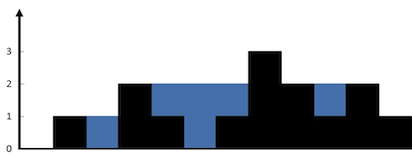
\includegraphics[height = 1in]{rainwatertrap}}
    \caption{Trapping Rain Water}
  \label{fig:rainwatertrap}
\end{figure}

Let $maxL_i$ be the $\max(A[:i])$; let $maxR_i$ be the $\max(A[i:n])$. The dp of obtaining max is trivial. 

The the total volume $vol$:
$$
vol = \sum_i(\max\big(0,\min(maxL_i, maxR_{i+1})-A[i]\big))
$$
\runinhead{Zigzag subsequence.} Find the max length zigzag subsequence which goes up and down alternately within the array $A$.

Let $U_i$ be the max length of zigzag subsequence end at $A_i \wedge$ going up.

Let $D_i$ be the max length of zigzag subsequence end at $A_i \wedge$ going down.
\begin{align*}
U_i &= max(D_j+1 \cdot \forall j < i) \text{ // if $A_i > A_j$} \\ 
D_i &= max(U_j+1 \cdot \forall j < i) \text{ // if $A_i < A_j$} 
\end{align*}

Notice in python implementation, don't use list comprehension since two states are interleaved and interdependent. 
\subsection{Automata}
\runinhead{Decode ways.} `A' encodes 1, `B' 2, ..., `Z' 26, Given an encoded message containing digits $S$, determine the total number of ways to decode it.

For example, given encoded message 12, it could be decoded as ``AB'' (1 2) or ``L'' (12). Thus, the number of ways decoding 12 is 2.

Let $F_i$ be number of decode ways for $s[:i]$. 

\begin{itemize}
\item If $s_{i-1}$ is 0, we only have one way to decode: $10$ or $20$.
$$
F_i = F_{i-2}
$$ 
\item If $s_{i-1}$ is not 0, we have two one ways to decode: 1) $1 \sim 9$; or 2) $10 \sim26$
$$
F_i = F_{i-1}+F_{i-2}
$$
\end{itemize}
\begin{python}
if s[i-1] != "0":
    F[i] = F[i-1]
    if 10 <= int(s[i-2]+s[i-1]) < 27:
        F[i] += F[i-2]
else:  # 0 is special
    if s[i-2] in ("1", "2"):
        F[i] = F[i-2]
    else:
        return 0
\end{python}
\runinhead{Regex}
\section{Graph}
\subsection{Binary Graph}
\runinhead{Maximal square.} Find the largest rectangle in the matrix:
\begin{lstlisting}
1 0 1 0 0
1 0 1 1 1
1 1 1 1 1
1 0 0 1 0
\end{lstlisting}
Let $F_{i, j}$ represents the max square's length ended at $mat_{i, j}$ (lower right
corner).
\begin{eqnarray*}
F_{i, j} = \left\{ \begin{array}{rl}
  \min\big(F_{i-1, j-1}, F_{i-1, j}, F_{i, j-1}\big)+1 &\mbox{// if $mat_{i, j}==1$}
\\
  0 &\mbox{// otherwise}
       \end{array} \right.
\end{eqnarray*}

\section{String}
\runinhead{Word break.} Given a string $s$ and a dictionary of words $dict$, determine if $s$ can be segmented into a space-separated sequence of $dict$ words.

Let $F_i$ be whether \pyinline{s[:i]} can be segmented. 
\begin{eqnarray*}
F_{i} = \left\{ \begin{array}{rl}
  F_{i-len(w)} &\mbox{// if $\exists w\in dict$, \pyinline{s[i-len(w):i]==w}}
\\
  false &\mbox{// otherwise}
       \end{array} \right.
\end{eqnarray*}
Return all such possible sentences. In original case, we use a bool array to record whether a dp could be segmented. Now we should use a vector for every dp to record how to construct that dp from another dp.

Let $F_i$ be all possible segmented words ends at \pyinline{s[i-1]}. $F_i$ is a list. $\exists F_i$ means $F_i$ is not empty.
\begin{eqnarray*}
F_{i} = \left\{ \begin{array}{rl}
  F_{i}+[w] &\mbox{// $\forall w\in dict\cdot$} \\
  & \mbox{ if \pyinline{s[i-len(w):i]==w} $\wedge\ \exists
F_{i-len(w)$ } \\
  F_{i}} &\mbox{// otherwise}
       \end{array} \right.
\end{eqnarray*}

Reconstruct the sentence from $F_i$. It is like building path for the tree. Using backtracking: 
\begin{python}
def build(self, dp, i, cur, ret):
    if cur_index == 0:
        ret.append(" ".join(list(cur)))
        return

    # backtracking
    for word in dp[i]:
        cur.appendleft(word)
        self.build(dp, i-len(word), cur, ret)
        cur.popleft()

\end{python}

\runinhead{Is palindrome.} Given a string $s$, use an array to determine whether $s[i:j]$.

Let $P_{i,j}$  indicates whether $s[i:j]$ is palindrome. We have one condition - whether the head and the end letter are equal: 
\begin{eqnarray*}
P_{i. j} = P_{i-1, j+1}\ \wedge\ s[i] = s[j-1]
\end{eqnarray*}

The code for palindrome dp is error-prone due to indexing. Notice that $i \in [0, n), j \in [i, n+1)$.
\begin{python}
n = len(s)
pa = [[False for _ in xrange(n+1)] for _ in xrange(n)]
for i in xrange(n):
    pa[i][i] = True
    pa[i][i+1] = True

for i in xrange(n-2, -1, -1):
    for j in xrange(i+2, n+1):
        pa[i][j] = pa[i+1][j-1] and s[i] == s[j-1]
\end{python}
\runinhead{Minimum palindrome cut.} Given a string s, partition s such that every substring of the partition is a palindrome. Return the minimum cuts needed for a palindrome partitioning of s.

Let $C_i$ be the min cut for $s[:i]$. We have 1 more cut from previous state to make $S[:i]$ palindrome. 
\begin{eqnarray*}
C_{i} = \left\{ \begin{array}{rl}
  \min\big(C[k]+1 \cdot \forall k<i \big) &\mbox{// if $s[k:i]$ is palindrome}
\\
  0 &\mbox{// otherwise}
       \end{array} \right.
\end{eqnarray*}
\begin{python}
def minCut(self, s):
  n = len(s)

  P = [[False for _ in xrange(n+1)] for _ in xrange(n+1)]
  for i in xrange(n+1):  # len 0
    P[i][i] = True
  for i in xrange(n):  # len 1
    P[i][i+1] = True

  for i in xrange(n, -1, -1):  # len 2 and above
    for j in xrange(i+2, n+1):
      P[i][j] = P[i+1][j-1] and s[i] == s[j-1]

  C = [i for i in xrange(n+1)]  # max is all cut
  for i in xrange(n+1):
    if P[0][i]:
      C[i] = 0
    else:
      C[i] = min(
          C[j] + 1
          for j in xrange(i)
          if P[j][i]
      )

  return C[n]
\end{python}
\runinhead{ab string.} Change the char in a str only consists of `a' and `b' to non-decreasing order. Find the min number of char changes. 

Two-state dp: `a' $\rightarrow$ `b' and  `b' $\rightarrow$ `a'. 1 cut into 2 segment.

\runinhead{abc string.} Follow up for ab string. Three-state dp: $chr \neq a, chr \neq b, chr \neq c$. 2 cuts into 3 segments.

\section{Divide \& Conquer}
\subsection{Tree}
\runinhead{Number of different BSTs.} It can be solved using Catalan number (Section \ref{section:catalanNumber}), but here goes the dp solution. 
\begin{lstlisting}
   1         3     3      2      1
    \       /     /      / \      \
     3     2     1      1   3      2
    /     /       \                 \
   2     1         2                 3
\end{lstlisting}

Let $F_i$ be the \#BSTs constructed from $i$ elements. The pattern is: 
\begin{align*}
F_3 = F_0*F_2 + F_1*F_1 + F_2*F_0
\end{align*}

Thus, in general, 
\begin{align*}
F_i = \sum(F_{j}*F_{i-1-j} \cdot \forall j< i)
\end{align*}

\subsection{Array}
\runinhead{Burst balloons.} Given $n$ balloons, indexed from 0 to $n-1$. Each balloon is painted with a number on it represented by array $A$. You are asked to burst all the balloons. If the you burst balloon i you will get \pythoninline{A[left] * A[i] * A[right]} coins. Here left and right are adjacent indices of i. After the burst, the left and right then becomes adjacent.

Find the maximum coins you can collect by bursting the balloons wisely.

\textbf{Core clues}:
\begin{enumerate}
\item Divide \& Conquer
\item Dividing Boundary 
\item Reverse Thinking: think about $n$ balloons if $A_i$ is the last one to burst, what now?
\end{enumerate}
Let $F_{i, j}$ be the max scores burst all over \pythoninline{A[i:j]}.

\begin{align*}
F_{i, j} = \max(F_{i,k} + A_{i-1}  A_k A_j + F_{k+1, j} \cdot \forall k)
\end{align*}
, where $k$ is the last one to burst.

\section{Backpack}
\subsection{Classical}
Given $n$ items with weight $w_i$ and value $v_i$, an integer $C$ denotes the size of a backpack. What is the max value you can fill this backpack?

Let $F_{i, c}$ be the max value we can carry for index $0..i$ with capacity $c$. We have 2 choices: take the $i$-th item or not.
\begin{eqnarray*}
F_{i, c}= \max\big(&&F_{i-1, c}, \\
&&F_{i-1, c-w_i}+v_i\big)
\end{eqnarray*}
Advanced backpack problem\footnote{\href{http://github.com/tianyicui/pack}{Nine Lectures in Backpack Problem}.}. 

\subsection{Sum}
\runinhead{k sum.} Given $n$ distinct positive integers, integer $k$ ($k \leq n$) and a number target. Find $k$ numbers where sum is target. Calculate the number of solutions. Since we only need the number of solutions, thus it can be solved using dp. If we need to enumerate all possible answers, need to do dfs instead. 

$$
sum{j \choose i} = v
$$

Let $F_{i, j, v}$ means the \#ways of selecting $i$ elements from the first $j$ elements so that their sum equals to $v$. $j$ is the scanning pointer.

You have two options: either select $A_{j-1}$ or not.
$$
F_{i, j, v} = F_{i-1, j-1, v-A_{j-1}} + F_{i, j-1, v}
$$
Time complexity: O(n^2 k)
\section{Local and Global Extremes}
\subsection{Long and short stocks}
\subsubsection{At most $k$ transactions}

The following formula derives from the question: Best Time to Buy and Sell Stock IV. Say you have an array for which the $i$-th element is the price of a given stock on day $i$. Design an algorithm to find the maximum profit. You may complete at most $k$ transactions. 

Let $local_{i, j}$ be the max profit with $j$ transactions with last transactions \textbf{ended at} day $i$. Let $global_{i, j}$ be the max profit with transactions \textbf{ended at} or \textbf{before} day $i$ with $j$ transactions. 

To derive transition function for $local$, for any given day $i$, you have two options: 1) transact in one day; 2) hold the stock one more day than previous and then transact. The latter option is equivalent to revert yesterday's transaction and instead transact today. 

To derive transition function for $global$, for any given day $i$, you have two options: 1) transact today; 2) don't transact today. 
\begin{eqnarray*}
&& local_{i,j} = \max\Big(global_{i-1.j-1}+\Delta, local_{i-1,j}+\Delta\Big) \nonumber \\
&& global_{i,j} = \max\Big(local_{i, j}, global_{i-1,j}\Big)
\end{eqnarray*}
, where $\Delta$ is the price change (i.e. profit) at day $i$.\\
Notice:
\begin{enumerate}
\item Consider opportunity costs and reverting transaction.
\item The global min is not $glocal[-1]$ but $\max\big(\{global[i]\}\big)$.
\item You must sell the stock before you buy again (i.e. you can not have higher than 1 in stock position). 
\end{enumerate}

\runinhead{Space optimization.}
\begin{eqnarray*}
&& local_{j} = \max\Big(global_{j-1} + \Delta, local_{j}+\Delta\Big)
\nonumber \\
&& global_{j} = \max\Big(local_{j}, global_{j}\Big)
\end{eqnarray*}

Notice,
\begin{enumerate}
\item Must iterate $j$ \textbf{backward}; otherwise we will use the updated value. 
\end{enumerate}

\runinhead{Alternative definitions.}
Other possible definitions: let $global_{i, j}$ be the max profit
with transactions ended at or before day $i$ with \textbf{up to} $j$ transactions. Then, 
\begin{eqnarray*}
&& local_{i,j} = \max\Big(global_{i-1.j-1} + \max(0, \Delta), local_{i-1,j}+\Delta\Big)
\nonumber \\
&& global_{i,j} = \max\Big(local_{i, j}, global_{i-1,j}\Big)
\end{eqnarray*}
and $global[-1]$ is the global max. 

The complexity of the alternative definitions is the same as the original definitions. The bottom line is that different definitions of states result in different transition functions.
\subsubsection{With cool down}

Find the maximum profit. You may complete as many transactions as you like with the following restrictions:
\begin{itemize}
\item You may not engage in multiple transactions at the same time (ie, you must sell the stock before you buy again).
\item After you sell your stock, you cannot buy stock on next day. (ie, cooldown 1 day)
\end{itemize}

Let $F_i$ be the max profit from day 0 to day $i$, selling stock at day $i$.

Let $M_i$ be the max profit from day 0 to day $i$.

For $F_i$, at each day $i$, you have two options: 1) Sell the stock that has been held for multiple days. 2) Sell the stock held for 1 day.
Notice the 1st option, it is equivalent to reverting the previous transaction, selling at day $i$ instead of day $i-1$.
\begin{eqnarray*}
F_{i}= \max\big(&&F_{i-1}+A_i-A_{i-1} \\
&&M_{i-2-CD}+A_i-A_{i-1}\big)
\end{eqnarray*}
, where $CD=1$, the cool down time. 

For $M_i$, simply, 
$$
M_i = \max(M_{i-1}, F_i)
$$


\section{Game theory - multi players}
Assumption: the opponent take the optimal strategy for herself. 

\subsection{Coin game}
\runinhead{Same side} There are $n$ coins with different value in a line. Two players take turns to take 1 or 2 coins from left side. The player who take the coins with the most value wins.

let $F_i^p$ represents maximum values he can get for index $i..last$, for the person p. There are 2 choices: take the $i$-th coin or take the $i$-th and $(i+1)$-th coin.
\begin{eqnarray*}
F_i^p = \max\big(&A_i&+S[i+1:]-F_{i+1}^{p'},  \\
&A_i&+A_{i+1}+S[i+2:]-F_{i+2}^{p'}\big)
\end{eqnarray*}
The above equation can be further optimized by merging the sum $S$.

\runinhead{Dual sides}There are n coins in a line. Two players take turns to take a coin from one of the ends of the line until there are no more coins left. The player with the larger amount of money wins.

let $F_{i, j}^p$ represents maximum values he can get for index $i..j$, for
the person p. There are 2 choices: take the $i$-th coin or take the $j$-th coin.
\begin{eqnarray*}
F_{i,j}^p = \max\big(&A_i&+S[i+1:j]-F_{i+1,j}^{p'},  \\
&A_j&+S[i:j-1]-F_{i,j-1}^{p'}\big)
\end{eqnarray*}
